\begin{figure}[htb!]
\centering
\begin{tabular}{lll}
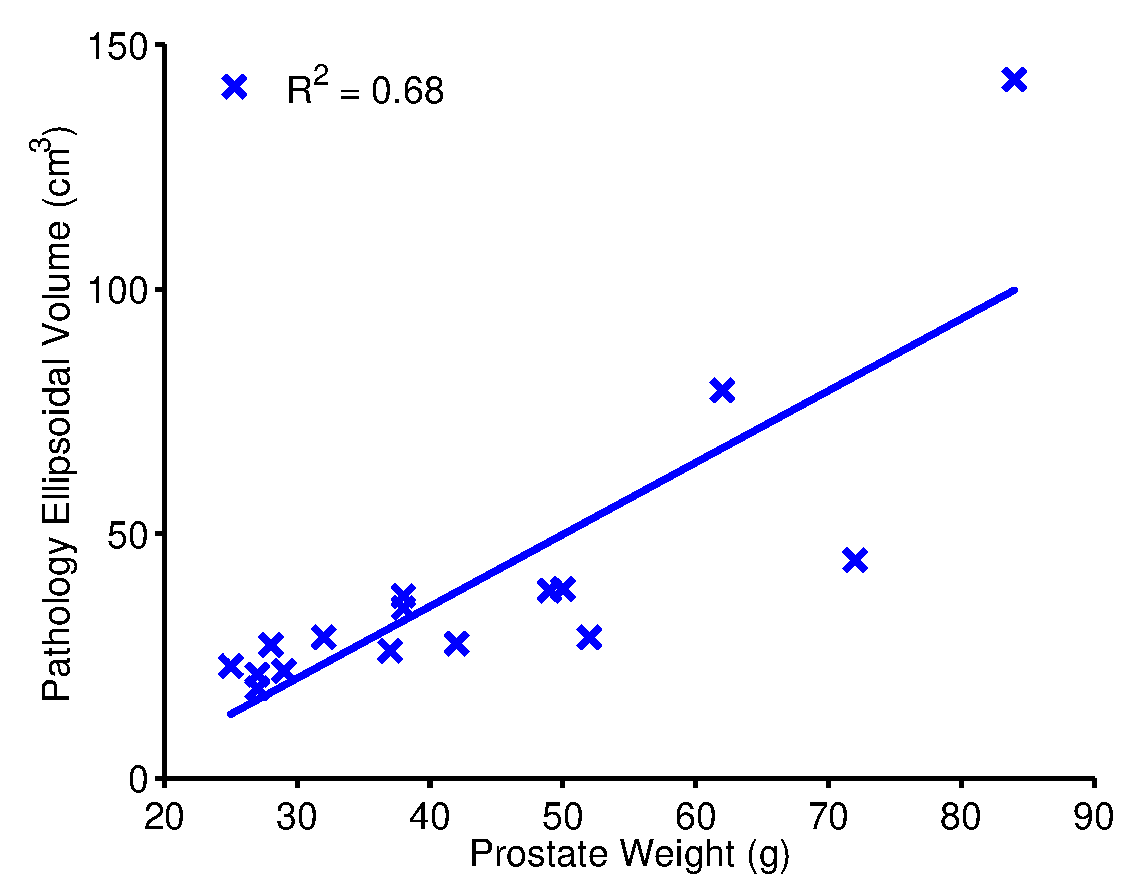
\includegraphics[width=0.3\linewidth]{figs/corr_path_vol_weight_vol} &
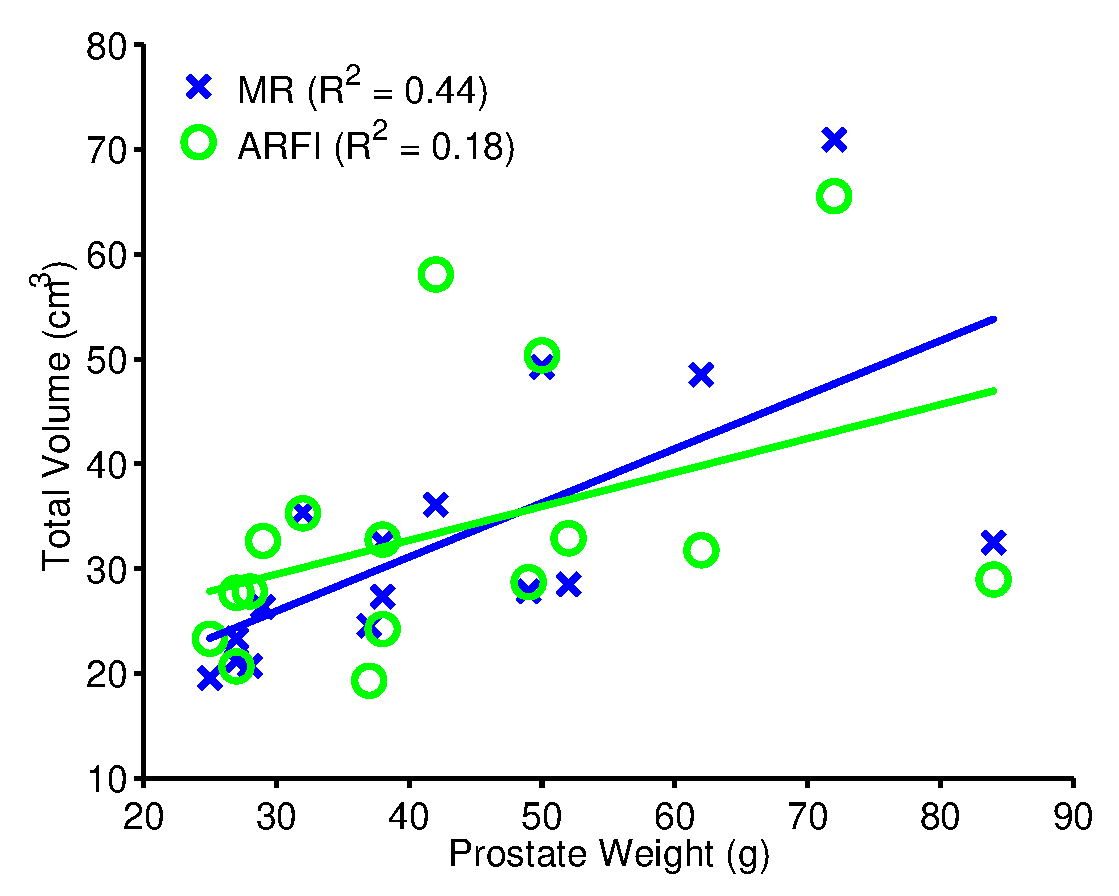
\includegraphics[width=0.3\linewidth]{figs/corr_weight_vol} &
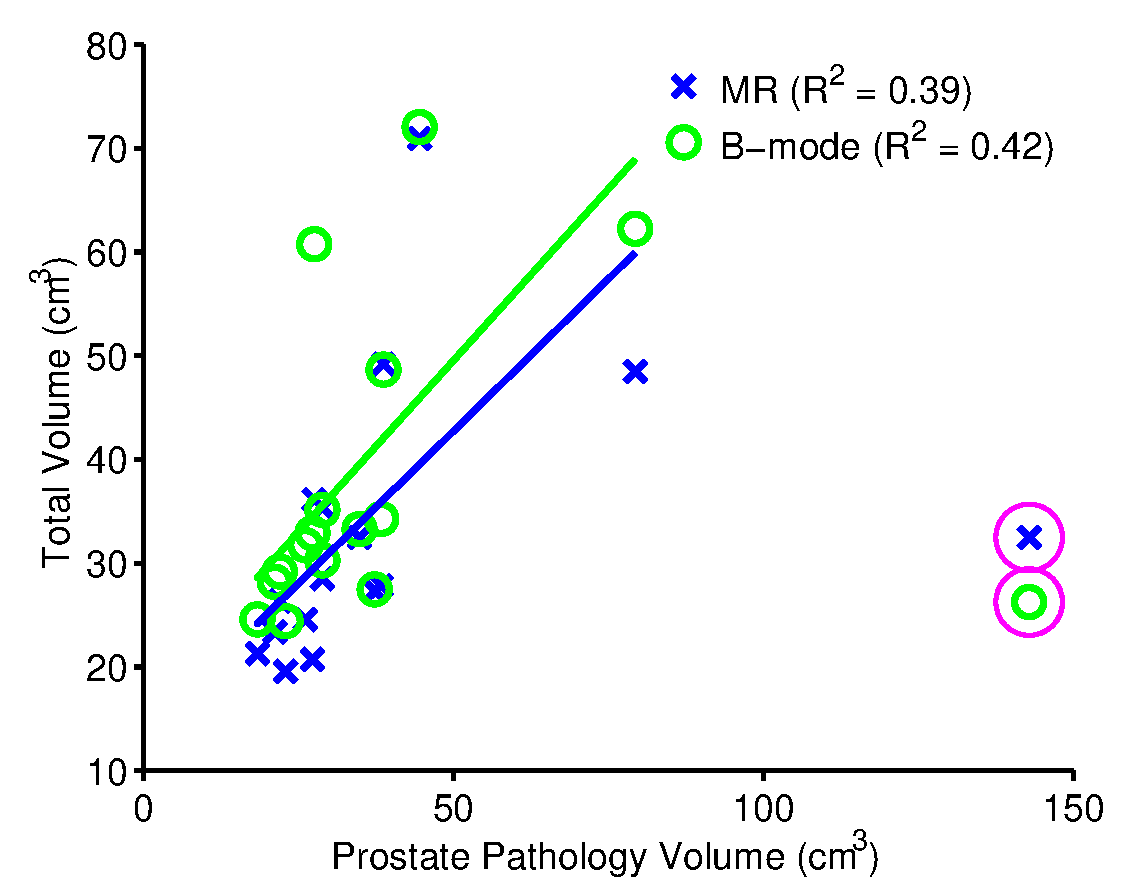
\includegraphics[width=0.3\linewidth]{figs/corr_pathVol_vol} \\
(a) Path Weight : Path Volume & (b) Image Volume : Prostate Weight & (c) Image Volume : Path Volume \\
\end{tabular}
\caption{Tri-axial pathology measurements were used to make an ellipsoidal
    prostate volume approximation based on gross pathology axis measurements,
    which was moderately well-correlated with the excised prostated weights (a,
    R$^2$ = 0.68).  T2WI MR (blue, X) showed a moderate correlation between the
    reconstructed volumes and prostate weight (R$^2$ = 0.44), while volumes
    reconstructed from ARFI images (green, O) showed weaker correlation (R$^2$
    = 0.21) (b).  Even weaker correlations existed between both T2WI MR and
    ARFI image volumens and approaximated ellipsoidal prostate pathology
    volumes (R$^2$ = 0.08 and 0.01, respectively) (c).}
\label{fig:mr_arfi_weight}
\end{figure}
